%%%%%%%%%%%%%%%%%%%%%%%%%%%%%%%%%%%%%%%%%%%%%%%%%%%%%%%%%%%%%%%%%%%%%%%%%%%%%%%%%%%%%%%%%%%%%%%%%%%%%%%%%%%
%                                           PACKAGES                                                      %
%%%%%%%%%%%%%%%%%%%%%%%%%%%%%%%%%%%%%%%%%%%%%%%%%%%%%%%%%%%%%%%%%%%%%%%%%%%%%%%%%%%%%%%%%%%%%%%%%%%%%%%%%%%
\documentclass[12pt, fleqn]{article}
\usepackage{amsmath, amsfonts, amsthm, amssymb, graphicx, enumitem, mathtools, MnSymbol, relsize, cancel}
\usepackage{siunitx}
\DeclareSIUnit\angstrom{\text{\AA}}
\usepackage{pdfpages}
\usepackage{graphicx}
\usepackage[utf8]{inputenc}
\usepackage{biblatex}
\usepackage{pythontex}
\usepackage{listings}
\usepackage[pdftex,pdfpagelabels,bookmarks,hyperindex,hyperfigures]{hyperref}
\hypersetup{colorlinks=true,allcolors=blue}
\usepackage{hypcap}
\usepackage{float}
\usepackage{geometry}
\geometry{margin=1in}
%%%%%%%%%%%%%%%%%%%%%%%%%%%%%%%%%%%%%%%%%%%%%%%%%%%%%%%%%%%%%%%%%%%%%%%%%%%%%%%%%%%%%%%%%%%%%%%%%%%%%%%%%%%
%                                           REFERENCE FILE                                                %
%%%%%%%%%%%%%%%%%%%%%%%%%%%%%%%%%%%%%%%%%%%%%%%%%%%%%%%%%%%%%%%%%%%%%%%%%%%%%%%%%%%%%%%%%%%%%%%%%%%%%%%%%%%
\usepackage[export]{adjustbox}
\graphicspath{{images/}}
%%%%%%%%%%%%%%%%%%%%%%%%%%%%%%%%%%%%%%%%%%%%%%%%%%%%%%%%%%%%%%%%%%%%%%%%%%%%%%%%%%%%%%%%%%%%%%%%%%%%%%%%%%%
%                                          PREPARE TITLE AND ABSTRACT                                     %
%%%%%%%%%%%%%%%%%%%%%%%%%%%%%%%%%%%%%%%%%%%%%%%%%%%%%%%%%%%%%%%%%%%%%%%%%%%%%%%%%%%%%%%%%%%%%%%%%%%%%%%%%%%
\title {
    \normalsize{UC Berkeley}\\
    \large{{EE140: Analog Integrated Circuit Devices\\Fall 2022\\Professor Ricky Muller\\}}
    \vspace{0.5ex}
    \Huge{Homework 9}
    \vspace{0.5ex}
}
\addbibresource{references.bib}
\author{Tarik Fawal}
\date{4 November 2022}
\usepackage{array}
\newcolumntype{C}[1]{>{\centering\arraybackslash}m{#1}}
\newcolumntype{N}{@{}m{0pt}@{}}
\begin{document}
%%%%%%%%%%%%%%%%%%%%%%%%%%%%%%%%%%%%%%%%%%%%%%%%%%%%%%%%%%%%%%%%%%%%%%%%%%%%%%%%%%%%%%%%%%%%%%%%%%%%%%%%%%%
%                                           GENERATE TITLE                                                %
%%%%%%%%%%%%%%%%%%%%%%%%%%%%%%%%%%%%%%%%%%%%%%%%%%%%%%%%%%%%%%%%%%%%%%%%%%%%%%%%%%%%%%%%%%%%%%%%%%%%%%%%%%%
\maketitle
\tableofcontents
\flushbottom
    \section*{Preface}
        \textit{\emph{This homework submission was created using \LaTeX.  The answers to questions were obtained through the course website, notes, textbook, and lecture videos.  I pledge that I have not plagiarized my solutions in any way, and the work presented here is my own.  References to any sources of material used in the solutions to this problem set are included at the end of this document.}}
\newpage
%%%%%%%%%%%%%%%%%%%%%%%%%%%%%%%%%%%%%%%%%%%%%%%%%%%%%%%%%%%%%%%%%%%%%%%%%%%%%%%%%%%%%%%%%%%%%%%%%%%%%%%%%%%
%                                           QUESTION 1                                                    %
%%%%%%%%%%%%%%%%%%%%%%%%%%%%%%%%%%%%%%%%%%%%%%%%%%%%%%%%%%%%%%%%%%%%%%%%%%%%%%%%%%%%%%%%%%%%%%%%%%%%%%%%%%%
\section{PSRR of the Two-Stage Amplifier}
\includepdf[pages=1-15]{Hw9_140.PDF}
\newpage
%%%%%%%%%%%%%%%%%%%%%%%%%%%%%%%%%%%%%%%%%%%%%%%%%%%%%%%%%%%%%%%%%%%%%%%%%%%%%%%%%%%%%%%%%%%%%%%%%%%%%%%%%%%
%                                           QUESTION 2                                                    %
%%%%%%%%%%%%%%%%%%%%%%%%%%%%%%%%%%%%%%%%%%%%%%%%%%%%%%%%%%%%%%%%%%%%%%%%%%%%%%%%%%%%%%%%%%%%%%%%%%%%%%%%%%%
\section{Miller Compensation of Two-Stage Amplifiers}
\includepdf[pages=16-26]{Hw9_140.PDF}
\newpage
%%%%%%%%%%%%%%%%%%%%%%%%%%%%%%%%%%%%%%%%%%%%%%%%%%%%%%%%%%%%%%%%%%%%%%%%%%%%%%%%%%%%%%%%%%%%%%%%%%%%%%%%%%%
%                                           QUESTION 3                                                    %
%%%%%%%%%%%%%%%%%%%%%%%%%%%%%%%%%%%%%%%%%%%%%%%%%%%%%%%%%%%%%%%%%%%%%%%%%%%%%%%%%%%%%%%%%%%%%%%%%%%%%%%%%%%
\section{Calculating Settling Errors}
    \begin{enumerate}[label=(\alph*)]
        %%%%%%%%%%%%%%%%%%%
        %    PART A       %
        %%%%%%%%%%%%%%%%%%%
        \item
        {
        Below is the code used for this part:\\[0.25cm]
        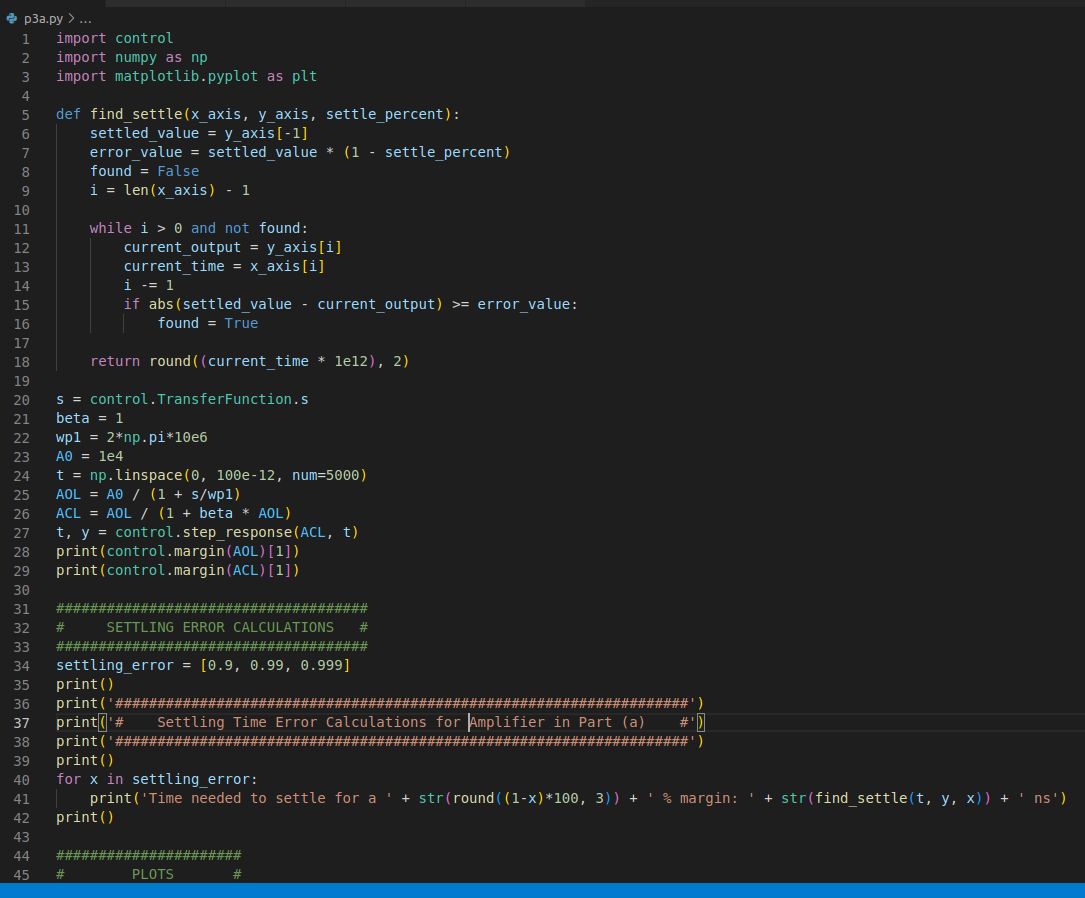
\includegraphics[scale=0.3, center]{p3a_code1.PNG}\\[0.25cm]
        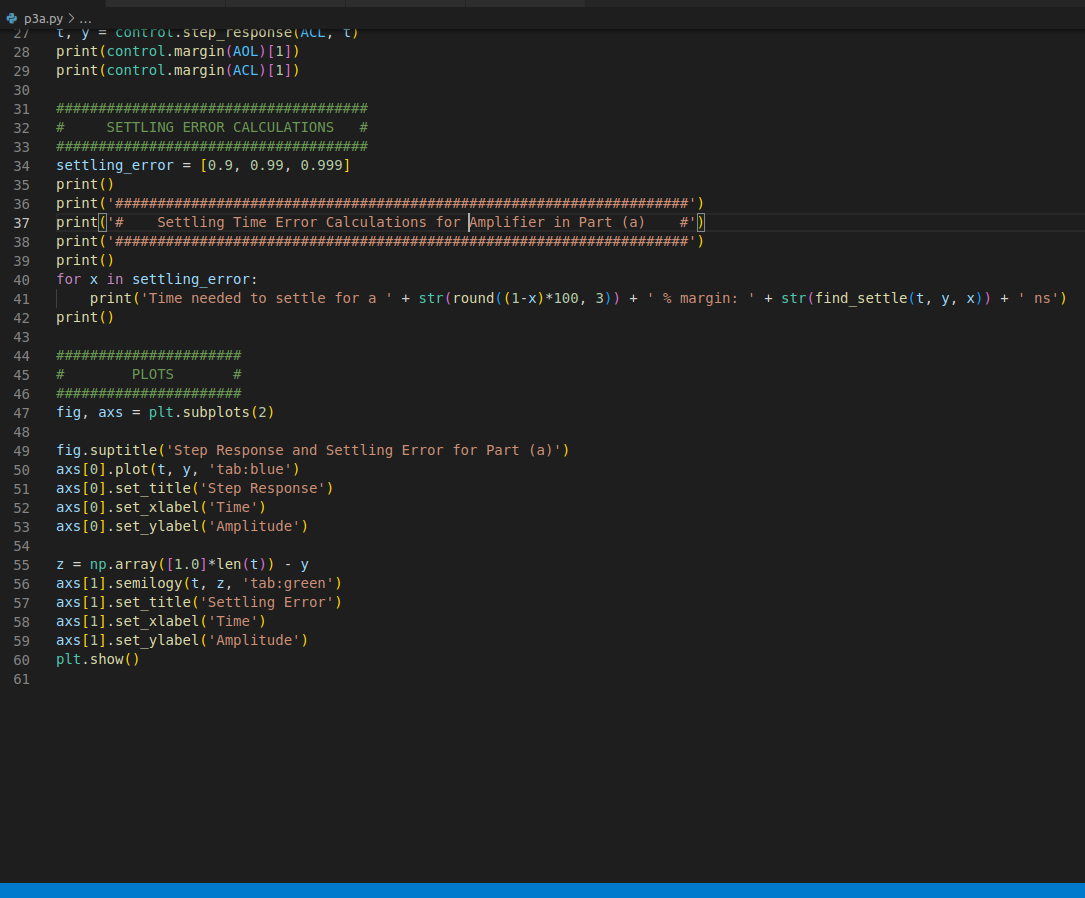
\includegraphics[scale=0.3, center]{p3a_code2.PNG}\\[0.25cm]
        \newpage
        Below is the plot and settling times:\\[0.25cm]
        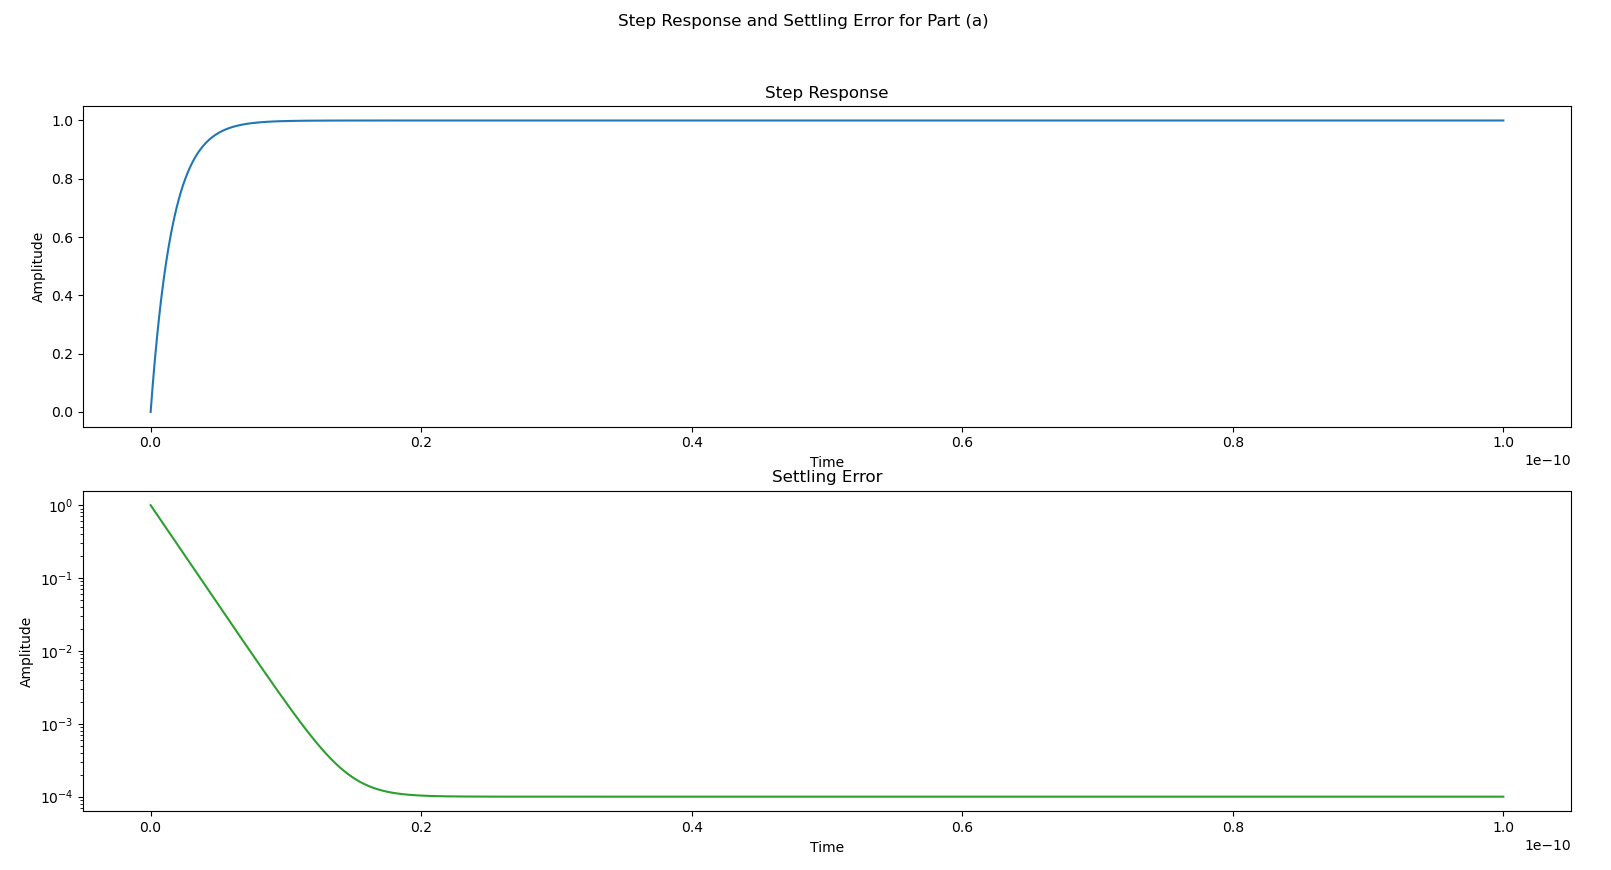
\includegraphics[scale=0.35, center]{p3a_plot.PNG}\\[0.25cm]
        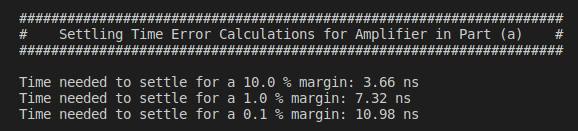
\includegraphics[scale=0.65, center]{p3a_settle.PNG}\\[0.25cm]
        }
        %%%%%%%%%%%%%%%%%%%
        %    PART B       %
        %%%%%%%%%%%%%%%%%%%
        \newpage
        \item
        {
        Below is the code used for this part:\\[0.25cm]
        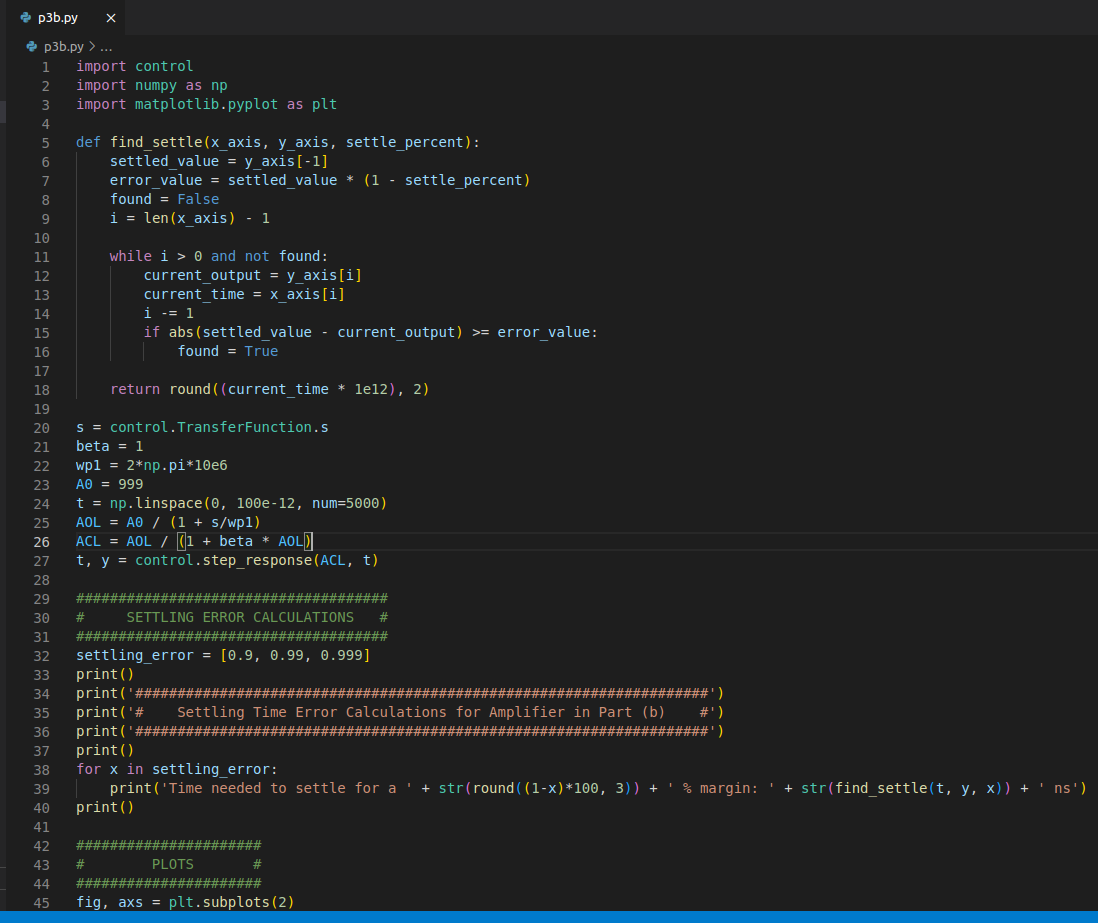
\includegraphics[scale=0.3, center]{p3b_code1.PNG}\\[0.25cm]
        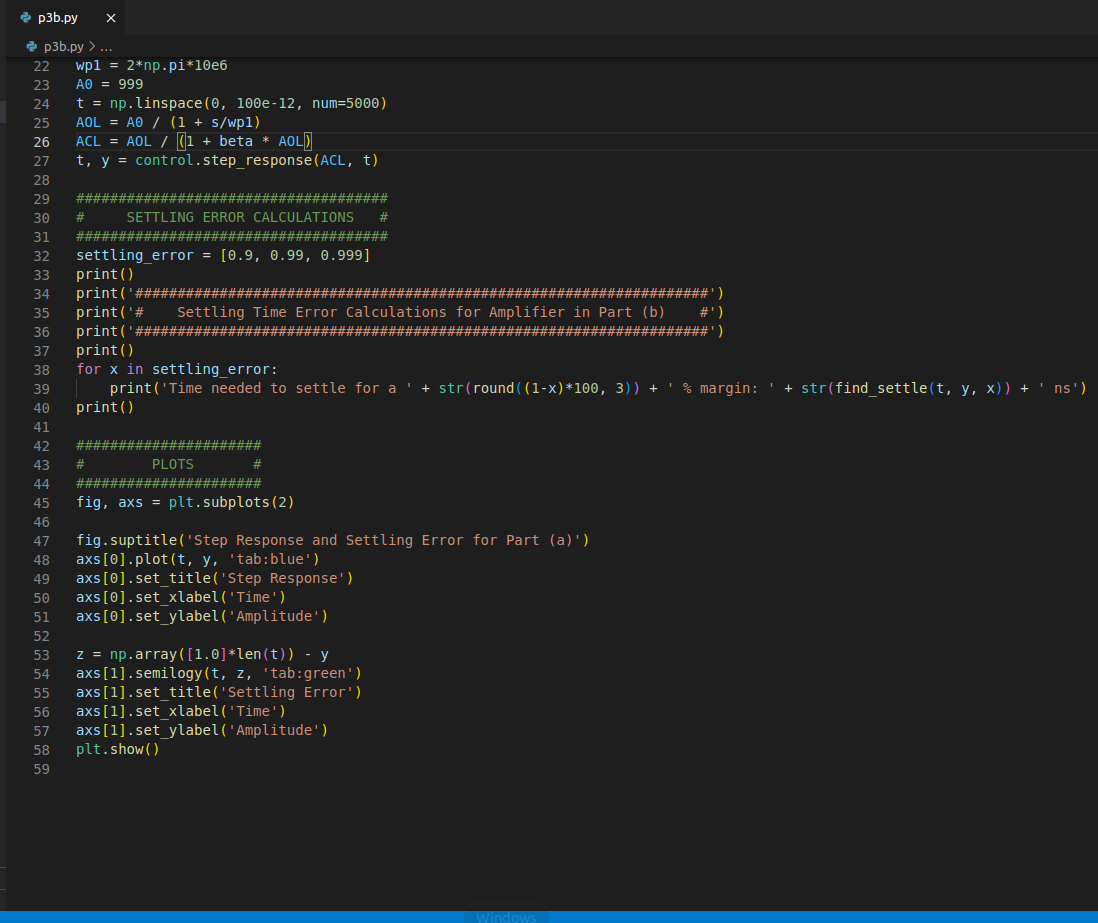
\includegraphics[scale=0.3, center]{p3b_code2.PNG}\\[0.25cm]
        \newpage
        Below is the plot and settling times:\\[0.25cm]
        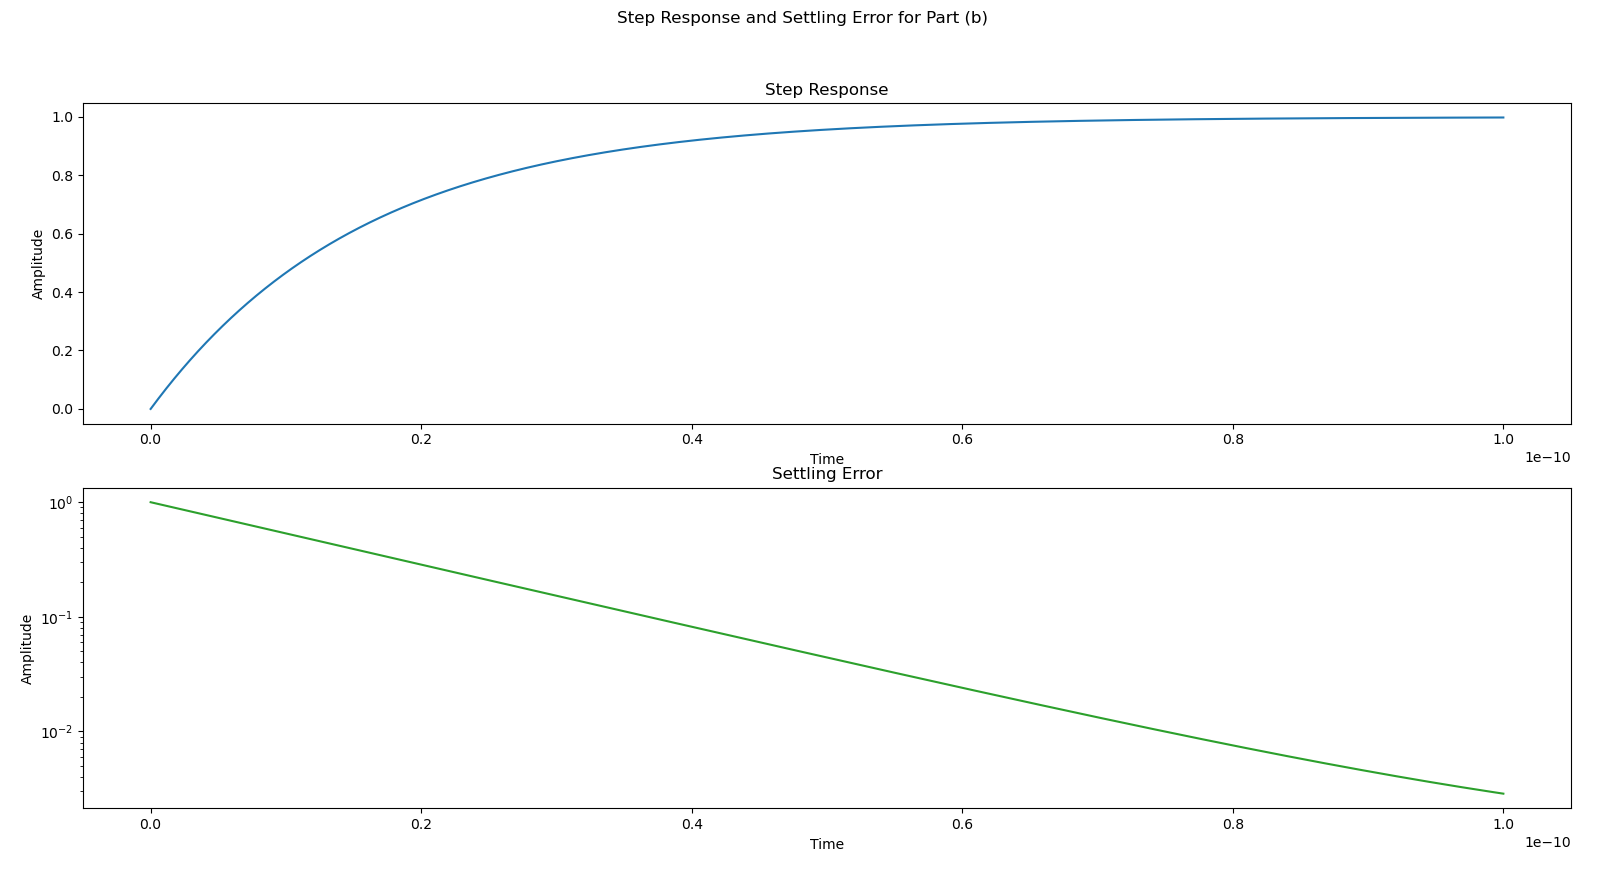
\includegraphics[scale=0.35, center]{p3b_plot.PNG}\\[0.25cm]
        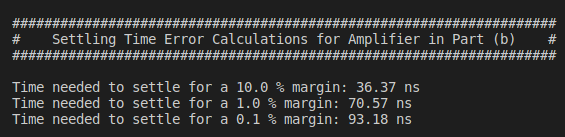
\includegraphics[scale=0.65, center]{p3b_settle.PNG}\\[0.25cm]
        }
        %%%%%%%%%%%%%%%%%%%
        %    PART C       %
        %%%%%%%%%%%%%%%%%%%
        \newpage
        \item
        {
        Below is a table of the results.\\[0.25cm]
        \begin{table}[H]
            \centering
            \setlength{\tabcolsep}{20pt}
            \renewcommand{\arraystretch}{1.5}
            \begin{tabular}{|l|c|c|}
                \hline
                \textbf{Error Margin} & \textit{Settling Time for Part (a)} & \textit{Settling Time for Part (b)}\\
                \hline
                \textit{10\%} & $36.81\,ns$ & $363.87\,ns$\\
                \hline
                \textit{1\%} & $73.41\,ns$ & $705.94\,ns$\\
                \hline
                \textit{0.1\%} & $110.02\,ns$ & $931.99\,ns$\\
                \hline
            \end{tabular}
        \end{table}
        The times all increased by approximately a factor of 10 when the gain was decreased.  I consider this to be a significant increase.  The shorter settling time is much closer to an ideal step response, whereas the longer settling time begins to look like a charging capacitor.\\[0.25cm]
        The reason that the settling time decreases with increasing gain, is because it takes much less input voltage to reach the final (ideal) level.  Another way to look at it is that a higher gain means a larger unity gain, and this results in a faster response time.
        }
        %%%%%%%%%%%%%%%%%%%
        %    PART D       %
        %%%%%%%%%%%%%%%%%%%
        \newpage
        \item
        {
        Below is the code used for this part:\\[0.25cm]
        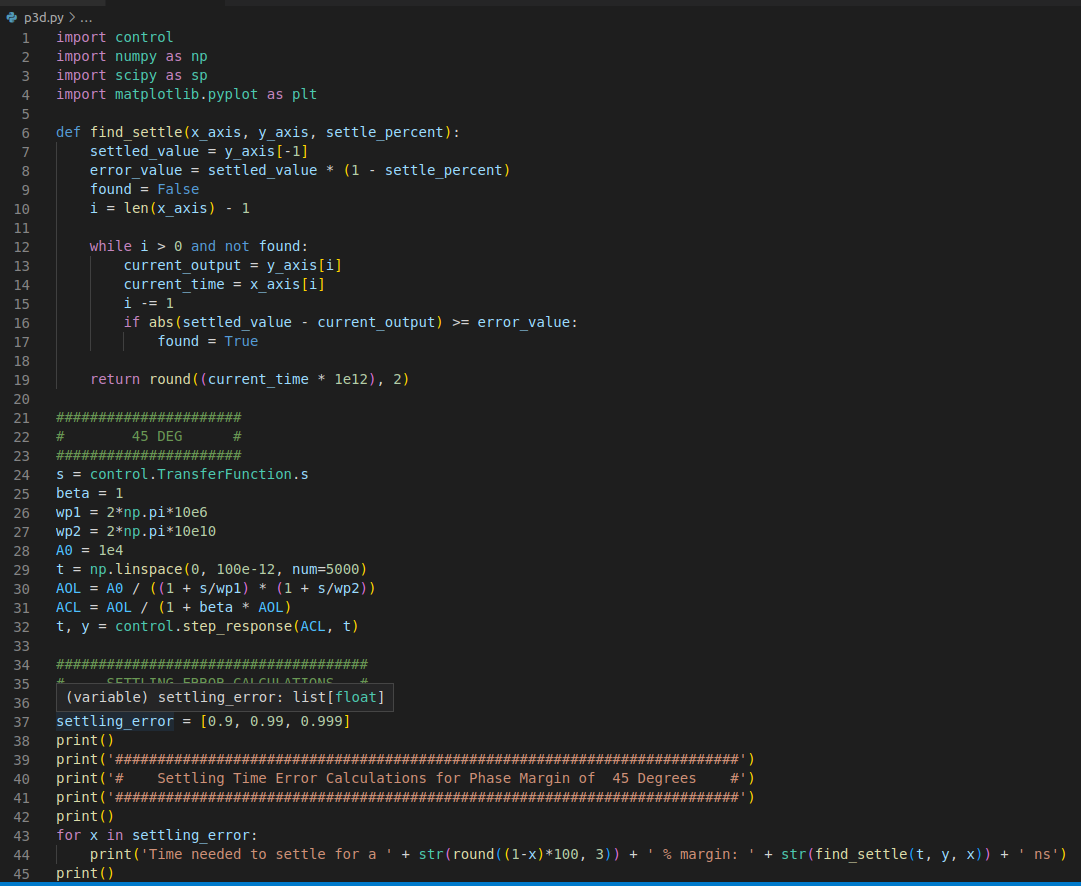
\includegraphics[scale=0.3, center]{p3d_code1.PNG}\\[0.25cm]
        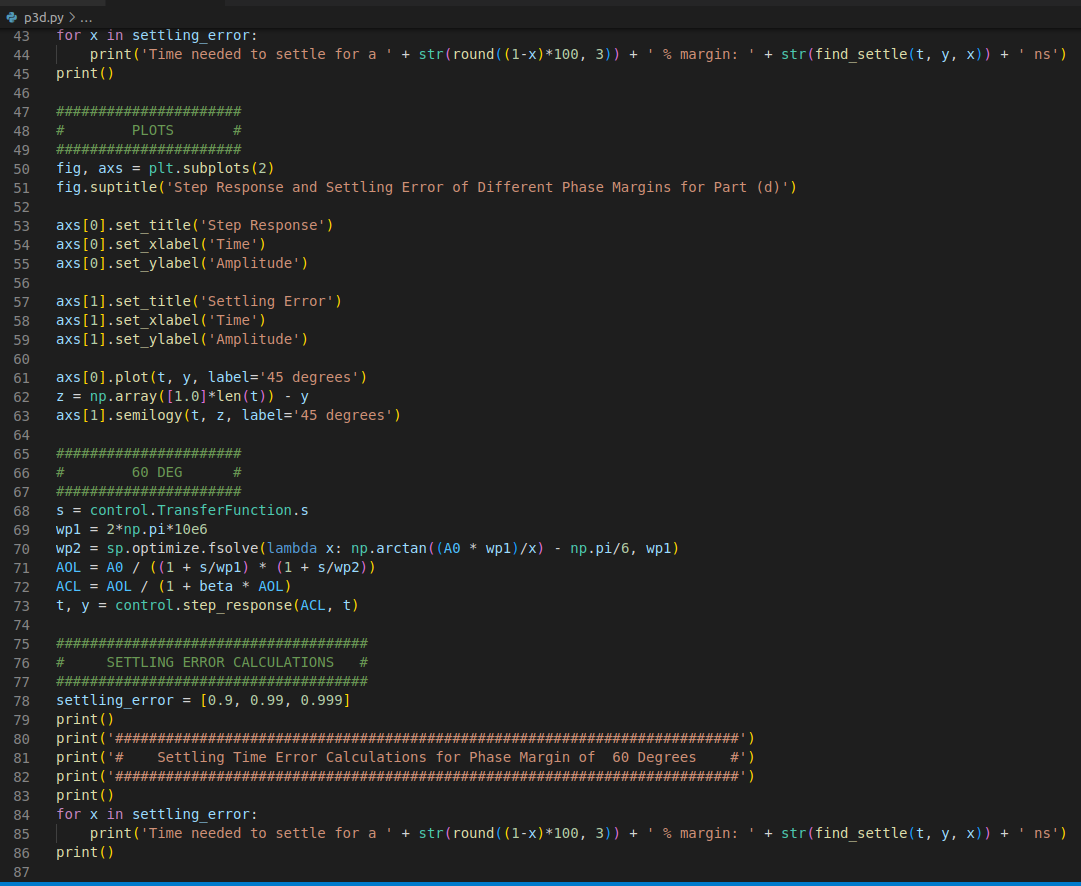
\includegraphics[scale=0.3, center]{p3d_code2.PNG}\\[0.25cm]
        \newpage
        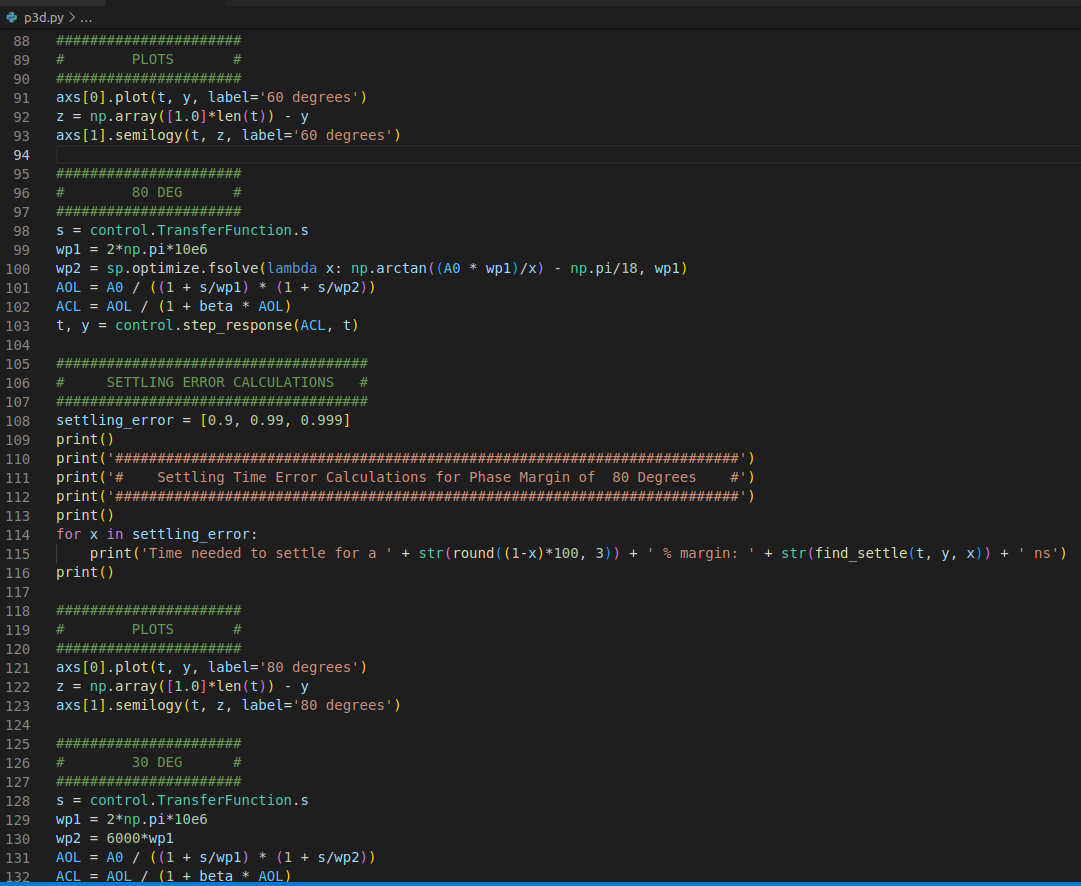
\includegraphics[scale=0.3, center]{p3d_code3.PNG}\\[0.25cm]
        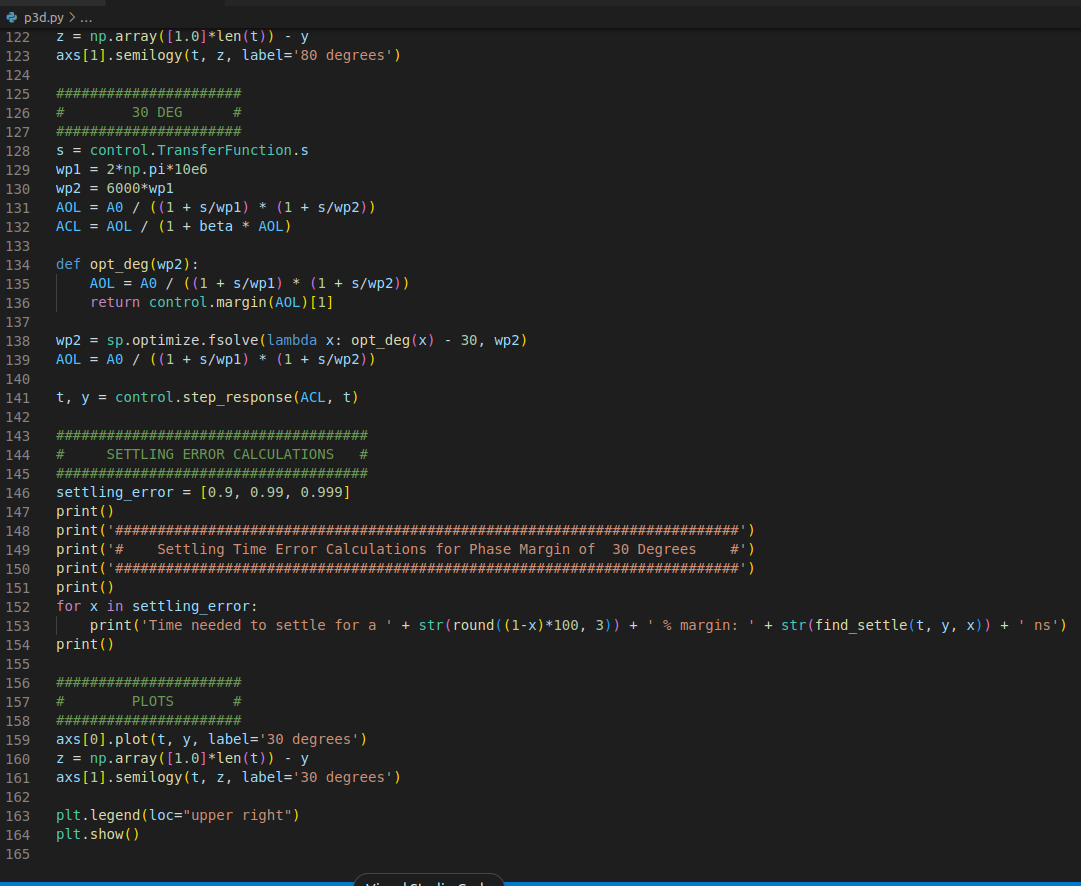
\includegraphics[scale=0.3, center]{p3d_code4.PNG}\\[0.25cm]
        \newpage
        Below is the plots and settling times:\\[0.25cm]
        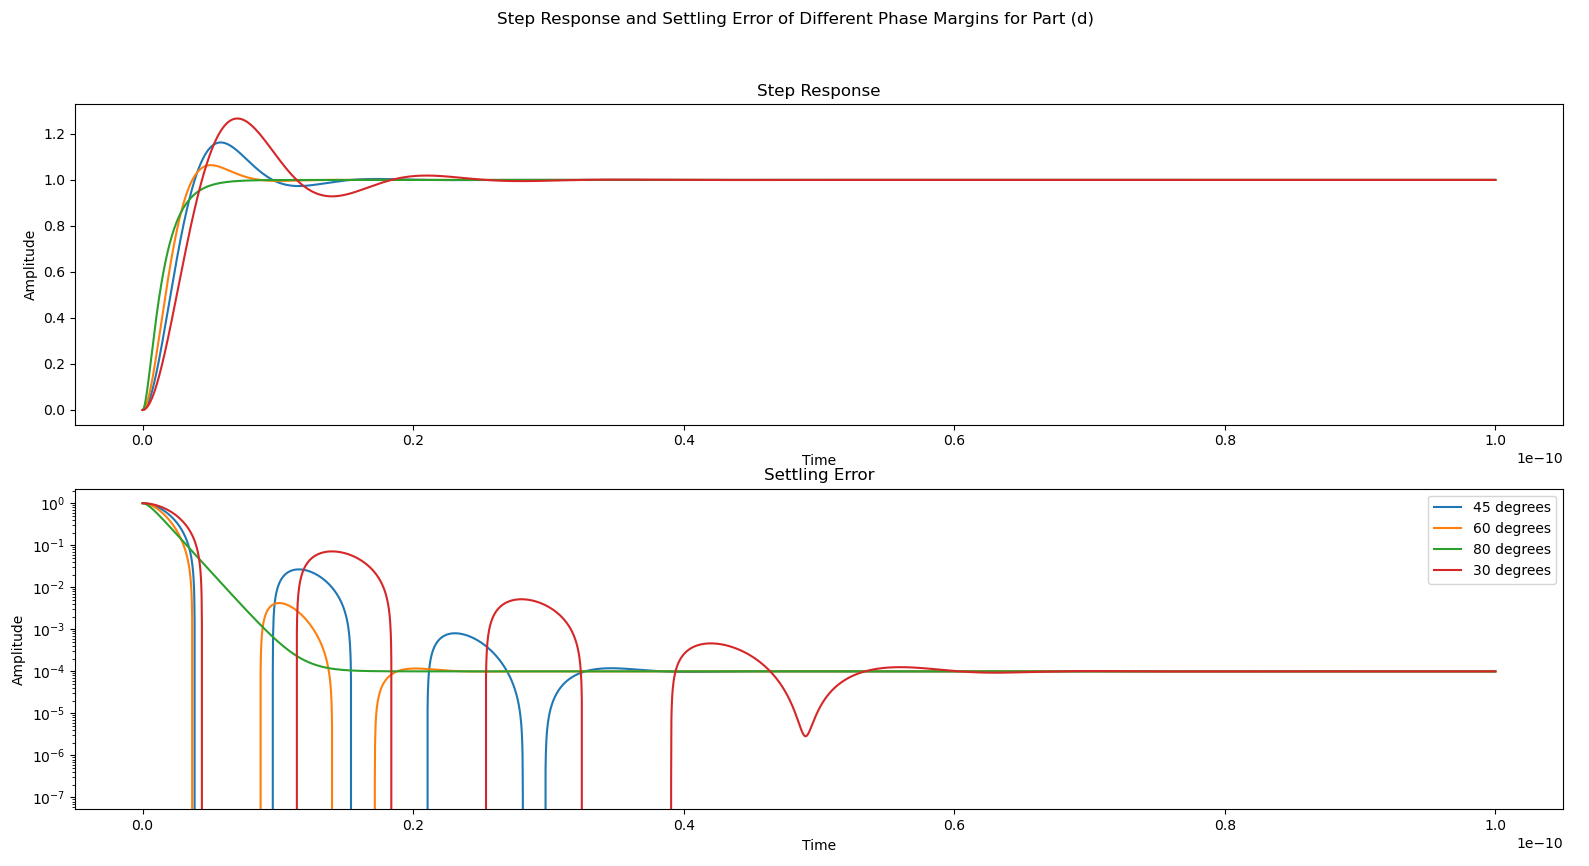
\includegraphics[scale=0.35, center]{p3d_plot.PNG}\\[0.25cm]
        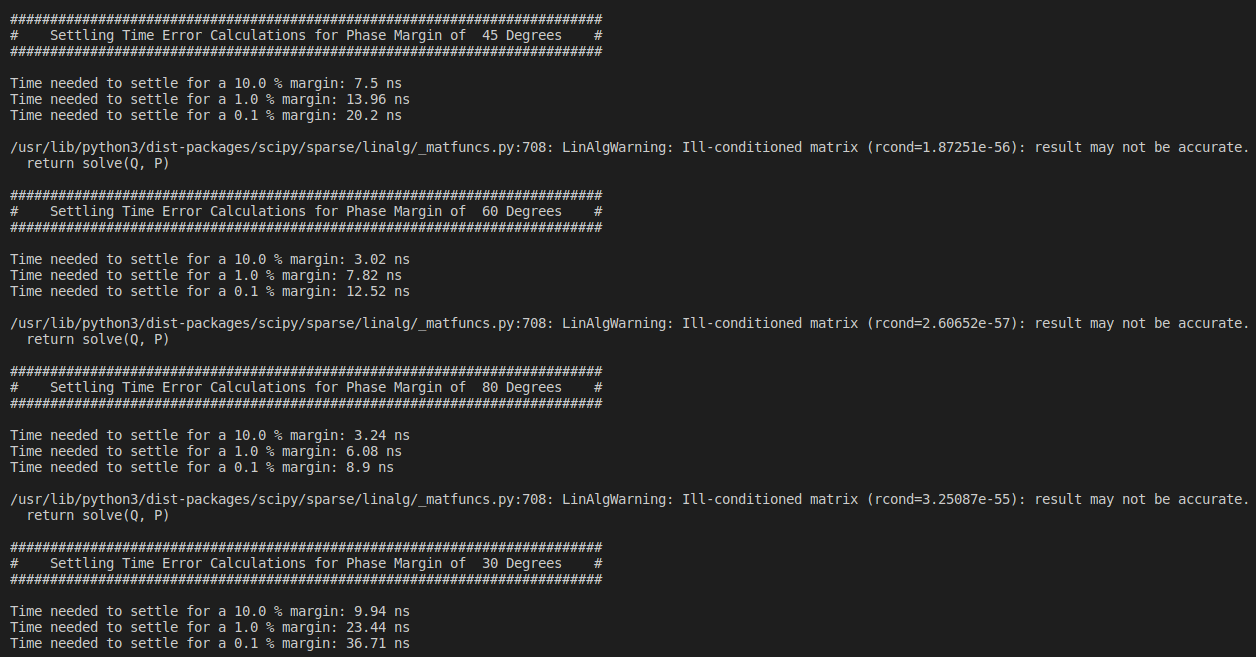
\includegraphics[scale=0.425, center]{p3d_settle.PNG}\\[0.25cm]
        }
        %%%%%%%%%%%%%%%%%%%
        %    PART E       %
        %%%%%%%%%%%%%%%%%%%
        \newpage
        \item
        {
        Below is the code used to find the optimal phase margins for each percent error.\\[0.25cm]
        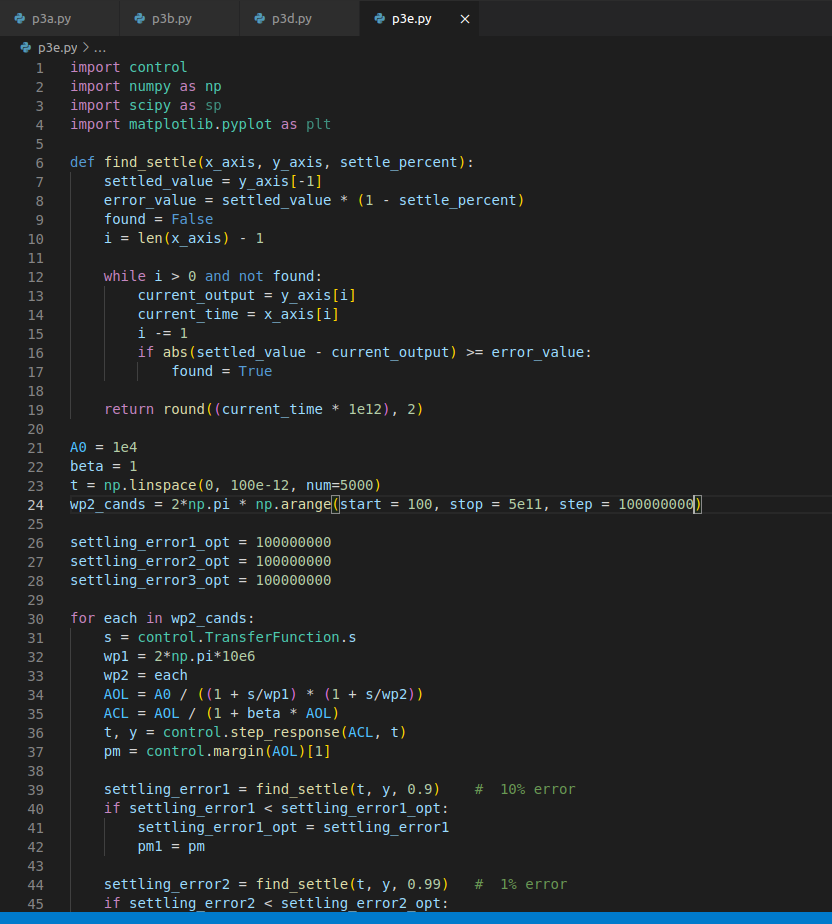
\includegraphics[scale=0.45, center]{p3e_code1.PNG}\\[0.25cm]
        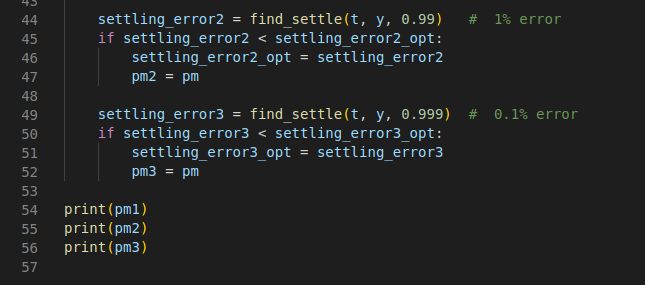
\includegraphics[scale=0.45, center]{p3e_code2.PNG}\\[0.25cm]
        Below is the snapshot of the results, which took about 5 minutes to run.\\[0.25cm]
        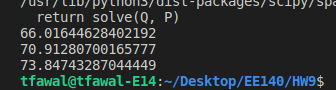
\includegraphics[scale=0.45, center]{p3e_res.PNG}\\[0.25cm]
        Below is a table of the results.\\[0.25cm]
        \begin{table}[H]
            \centering
            \setlength{\tabcolsep}{20pt}
            \renewcommand{\arraystretch}{1.5}
            \begin{tabular}{|l|c|}
                \hline
                \textbf{Error Margin}  &  \textit{Optimal Phase Margin}\\
                \hline
                \textit{10\%} & $\approx 62^\circ$\\
                \hline
                \textit{1\%} & $\approx 71^\circ$\\
                \hline
                \textit{0.1\%} & $\approx 74^\circ$\\
                \hline
            \end{tabular}
        \end{table}
        \underline{\textbf{\textit{Comments}}}\\[0.25cm]
        It is interesting to note that the optimal phase margin increases as the error margin decreases.  This is because with a larger error margin, the oscillations from the circuit ringing are still within the bounds of error.  Thus, the settling time occurs sooner than it would with a damped response.
        }
    \end{enumerate}
\newpage
%%%%%%%%%%%%%%%%%%%%%%%%%%%%%%%%%%%%%%%%%%%%%%%%%%%%%%%%%%%%%%%%%%%%%%%%%%%%%%%%%%%%%%%%%%%%%%%%%%%%%%%%%%%
%                                             APPENDIX                                                    %
%%%%%%%%%%%%%%%%%%%%%%%%%%%%%%%%%%%%%%%%%%%%%%%%%%%%%%%%%%%%%%%%%%%%%%%%%%%%%%%%%%%%%%%%%%%%%%%%%%%%%%%%%%%
\appendix
%%%%%%%%%%%%%%%%%%%%%%%%%%%%%%%%%%%%%%%%%%%%%%%%%%%%%%%%%%%%%%%%%%%%%%%%%%%%%%%%%%%%%%%%%%%%%%%%%%%%%%%%%%%
%                                APPENDIX A: GLOSSARY OF EQUATIONS                                        %
%%%%%%%%%%%%%%%%%%%%%%%%%%%%%%%%%%%%%%%%%%%%%%%%%%%%%%%%%%%%%%%%%%%%%%%%%%%%%%%%%%%%%%%%%%%%%%%%%%%%%%%%%%%
\newpage
\section{Appendix: Glossary of Equations}
    \begin{flalign}
        &&\Aboxed{\phi_{bi} &= \frac{kT}{q} \cdot ln\;\bigg( \frac{N_D \cdot N_A}{{n_i}^2} \bigg)}
        &&\textit{Built-in potential, $PN$-junction}
        \label{eq:phi_bi}
    \end{flalign}

    \begin{flalign}
        &&\Aboxed{W_{dep} &= \sqrt{\frac{2\epsilon_s \left(\phi_{bi} - V_{applied}\right)}{q}
                        \cdot \Bigg( \frac{1}{N_A} + \frac{1}{N_D} \Bigg)}}
        &&\textit{Depletion region width, total}
        \label{eq:total_dep}
    \end{flalign}        

    \begin{flalign}
        &&\Aboxed{C_{dep} &= A \left(\frac{\epsilon_s}{W_{dep}}\right)}
        &&\textit{Junction capacitance}
        \label{eq:junc_cap}
    \end{flalign}

    \begin{flalign}
        &&\Aboxed{I_{DS,sat} &= \left(\frac{W}{2L}\right) \mu_n\,C_{ox}
                         {\big(V_{GS} - V_{T_n}\big)}^2 (1 + \lambda V_{DS})}
        &&\textit{$NMOS$ saturation current}
        \label{eq:mosfet_ids_nmos_sat}\\[0.25cm]
        &&\Aboxed{I_{DS,tri} &= \left(\frac{W}{L}\right) \mu_n\,C_{ox}
                            \left(V_{GS} - V_{T_n} - \frac{V_{DS}}{2}\right) V_{DS}}
        &&\textit{$NMOS$ triode current}
        \label{eq:mosfet_ids_nmos_tri}\\[0.25cm]
        &&\Aboxed{I_{SD,sat} &= \left(\frac{W}{2L}\right) \mu_p\,C_{ox}
                         {\big(V_{SG} - \left|V_{T_p}\right|\big)}^2 (1 + \lambda V_{SD})}
        &&\textit{$PMOS$ saturation current}
        \label{eq:mosfet_ids_pmos_sat}\\[0.25cm]
        &&\Aboxed{I_{SD,tri} &= \left(\frac{W}{L}\right) \mu_p\,C_{ox}
                            \left(V_{SG} - \left|V_{T_p}\right| - \frac{V_{SD}}{2}\right) V_{SD}}
        &&\textit{$PMOS$ triode current}
        \label{eq:mosfet_ids_pmos_tri}
    \end{flalign}

    \begin{flalign}
        &&\Aboxed{r_o &= \frac{1}{\frac{W\,\mu\,C_{ox}}{2L}{(V_{GS} - V_T)}^2\,\lambda}
        \approx \frac{1}{\lambda\,I_{DS}}}
        &&\textit{Output resistance for MOSFET}
        \label{eq:mos_outresistance}
    \end{flalign}

    \begin{flalign}
        &&\Aboxed{g_m &= \left(\frac{W}{L}\right)\mu\,C_{ox}(V_{{DS}_{sat}})
        = \sqrt{\left(\frac{2W}{L}\right)\mu\,C_{ox} I_{DS}}
        = \frac{2 \cdot I_{DS}}{V_{GS} - V_T}}
        &&\textit{Transconductance for MOSFET}
        \label{eq:mos_transconductance}
    \end{flalign}

    \begin{flalign}
        &&\Aboxed{V_{GS} = V_T + \sqrt{\frac{2\,I_{DS}}{\frac{W}{L} \mu C_{ox}}} = V_T + V_{OD}}
        &&\textit{Gate-source condition, diode-connected MOSFET}
        \label{eq:mos_gate_cond}
    \end{flalign}
%%%%%%%%%%%%%%%%%%%%%%%%%%%%%%%%%%%%%%%%%%%%%%%%%%%%%%%%%%%%%%%%%%%%%%%%%%%%%%%%%%%%%%%%%%%%%%%%%%%%%%%%%%%
%                                APPENDIX B: GLOSSARY OF TABLES                                           %
%%%%%%%%%%%%%%%%%%%%%%%%%%%%%%%%%%%%%%%%%%%%%%%%%%%%%%%%%%%%%%%%%%%%%%%%%%%%%%%%%%%%%%%%%%%%%%%%%%%%%%%%%%%
\newpage
\section{Appendix: Glossary of Tables}
    \begin{table}[H]
    \centering
    \setlength{\tabcolsep}{20pt}
    \renewcommand{\arraystretch}{1.5}
    \begin{tabular}{|l|c|c|c|}
        \hline
        \textbf{Transistor Type}  &  \textbf{Cut-off} & \textbf{Triode} & \textbf{Saturation}\\
        \hline
        \textit{NMOS} & $V_{GS} \leq V_{T_n}$
                        & $V_{DS} \leq V_{GS} - V_{T_n}$
                        & $V_{DS} > V_{GS} - V_{T_n}$\\
        \hline
        \textit{PMOS} & $V_{SG} \leq \left|V_{T_p}\right|$
                        & $V_{SD} \leq V_{SG} - \left|V_{T_p}\right|$
                        & $V_{SD} > V_{SG} - \left|V_{T_p}\right|$\\
        \hline
    \end{tabular}
    \caption{Conditions for MOSFET regions of operation.
    \label{tab:mosfet_op}} 
    \end{table}

    \begin{table}[H]
    \centering
    \setlength{\tabcolsep}{20pt}
    \renewcommand{\arraystretch}{1.5}
    \begin{tabular}{|l|c|c|}
        \hline
        \textbf{Description}  &  \textbf{Symbol} & \textbf{Value}\\
        \hline
        Elementary charge & $q$ & $\num{1.60218e-19}\,C$\\
        \hline
        Electron volt & $eV$ & $\num{1.60218e-19}\,J$\\
        \hline
        Boltzmann's constant & $k$ & $\num{1.38066e-23}\,J/K$\\
        \hline
        Free electron mass & $m_0$ & $\num{9.1095e-31}\,kg$\\
        \hline
        Permittivity in vacuum & $\epsilon_0$ & $\num{8.85418e-12}\,F/m$\\
        \hline
        Planck's constant & $h$ & $\num{6.62617e-34}\,J \cdot s$\\
        \hline
        Reduced Planck's constant ($h/2\pi$) & $\hbar$ & $\num{1.05458e-34}\,J \cdot s$\\
        \hline
        Speed of light in vacuum & $c$ & $\num{2.99792e8}\,m/s$\\
        \hline
        Thermal voltage at $T=300^{\circ}K$ & $kT/q$ & $0.0259\,V$\\
        \hline
        Wavelength of 1-$eV$ photon & $\lambda$ & $1.23977\,\mu m$\\
        \hline
    \end{tabular}
    \caption{Physical constants.
    \label{tab:phys_const}} 
    \end{table}
\newpage
    \begin{table}[H]
    \centering
    \setlength{\tabcolsep}{20pt}
    \renewcommand{\arraystretch}{1.5}
    \begin{tabular}{|l|c|c|}
        \hline
        \textbf{Quantity}  &  \textbf{Symbol} & \textbf{Value/Dimension}\\
        \hline
        Meter & $m$ & $1\,m = 10^2\,cm$\\
        \hline
        Millimeter & $mm$ & $1\,mm = 10^{-1}\,cm = 10^{-3}\,m$\\
        \hline
        Micrometer, micron & $\mu m$ & $1\,\mu m = 10^4\,\text{\AA} = 10^3\,mm = 10^{-4}\,cm$\\
        \hline
        Nanometer & $nm$ & $1\,nm = 10\,\text{\AA} = 10^{-3}\,\mu m = 10^{-7}\,cm$\\
        \hline
        Angstrom & $\text{\AA}$ & $1\,\text{\AA} = 10^{-4}\,\mu m = 10^{-8}\,cm = 10^{-10}\,m$\\
        \hline
        Electron volt & $eV$ & $1\,eV = \num{1.60218e-19}\,J$\\
        \hline
        Electric charge (Coulomb) & $C$ & $A \cdot s$\\
        \hline
        Current (Ampere) & $A$ & $C/s$\\
        \hline
        Frequency (Hertz) & $Hz$ & $1/s$\\
        \hline
        Energy (Joule) & $J$ & $N \cdot m$\\
        \hline
        Power (Watt) & $W$ & $J/s$\\
        \hline
        Potential (Volt) & $V$ & $J/C$\\
        \hline
        Conductance (Siemens) & $S$ & $A/V$\\
        \hline
        Resistance (Ohm) & $\Omega$ & $V/A$\\
        \hline
        Capacitance (Farad) & $F$ & $C/V$\\
        \hline
    \end{tabular}
    \caption{Unit conversions.
    \label{tab:unit_conv}} 
    \end{table}
\newpage
%%%%%%%%%%%%%%%%%%%%%%%%%%%%%%%%%%%%%%%%%%%%%%%%%%%%%%%%%%%%%%%%%%%%%%%%%%%%%%%%%%%%%%%%%%%%%%%%%%%%%%%%%%%
%                                           BIBLIOGRAPHY                                                  %
%%%%%%%%%%%%%%%%%%%%%%%%%%%%%%%%%%%%%%%%%%%%%%%%%%%%%%%%%%%%%%%%%%%%%%%%%%%%%%%%%%%%%%%%%%%%%%%%%%%%%%%%%%%
\newpage
\addcontentsline{toc}{section}{References}
\emergencystretch=2em
\nocite{*}
\printbibliography
%%%%%%%%%%%%%%%%%%%%%%%%%%%%%%%%%%%%%%%%%%%%%%%%%%%%%%%%%%%%%%%%%%%%%%%%%%%%%%%%%%%%%%%%%%%%%%%%%%%%%%%%%%%
%                                           END OF DOCUMENT                                               %
%%%%%%%%%%%%%%%%%%%%%%%%%%%%%%%%%%%%%%%%%%%%%%%%%%%%%%%%%%%%%%%%%%%%%%%%%%%%%%%%%%%%%%%%%%%%%%%%%%%%%%%%%%%
\end{document}
